\documentclass[11pt,reqno,final]{amsart}

\pdfcompresslevel=0
\pdfobjcompresslevel=0

\usepackage[dvipsnames]{xcolor}% adds colors
\usepackage{amsmath, amsthm}% {amsfonts, amssymb}

% New Characters
\usepackage[latin1]{inputenc}%
\usepackage[T1]{fontenc}

\usepackage{MnSymbol}
\usepackage[normalem]{ulem}% underlining

\usepackage[theoremfont, largesc]{newpxtext} % different text,math font
\usepackage{newpxmath}

\makeatletter
\DeclareMathRadical{\sqrtsign}{symbols}{112}{largesymbols}{112}
% \let\sqrt=\undefined
% \DeclareRobustCommand\sqrt{\@ifnextchar[\@sqrt{\mathpalette\@x@sqrt}]}
% \def\@x@sqrt#1#2{%
%  \setbox\z@\hbox{$\m@th#1\sqrtsign{\mkern1mu #2}$}
%  \mkern3mu\box\z@}
\makeatother




% Page Typesetting
\usepackage[final]{microtype}
\usepackage{relsize}
\usepackage[margin=1in]{geometry}
\usepackage{framed}
\usepackage{tikz}

\usepackage{csquotes}

\usepackage{setspace}
\onehalfspacing

\usepackage{hyperref}
\hypersetup{
  final,
  pdftitle={Math 135 - Chain Rule},
  pdfauthor={Bonventre}, 
  linktoc=page,
  pagebackref,
  colorlinks=true,
  citecolor=PineGreen,
  linkcolor=PineGreen,
  linkbordercolor=PineGreen,
}


% Internal References

\usepackage[inline,shortlabels]{enumitem}

% \numberwithin{equation}{section} 
\numberwithin{figure}{section}

\usepackage[nameinlink,capitalise,noabbrev]{cleveref}

\crefname{equation}{}{} % get \cref to behave as \eqref

% \theoremstyle{plain} % bold name, italic text
\newtheorem{theorem}[equation]{Theorem}%
\newtheorem*{theorem*}{Theorem}%
\newtheorem{lemma}[equation]{Lemma}%
\newtheorem{proposition}[equation]{Proposition}%
\newtheorem{corollary}[equation]{Corollary}%
\newtheorem{conjecture}[equation]{Conjecture}%
\newtheorem*{conjecture*}{Conjecture}%
\newtheorem{claim}[equation]{Claim}%
\newtheorem{question}{Question}

\theoremstyle{definition} % bold name, plain text
\newtheorem{definition}[equation]{Definition}%
\newtheorem*{definition*}{Definition}%
\newtheorem{example}[equation]{Example}%
\newtheorem*{example*}{Example}%
\newtheorem{remark}[equation]{Remark}%
\newtheorem{notation}[equation]{Notation}%
\newtheorem{convention}[equation]{Convention}%
\newtheorem{assumption}[equation]{Assumption}%
\newtheorem{exercise}[question]{Exercise}

% ---------- macros
\newcommand{\set}[1]{\left\{#1\right\}}%
\newcommand{\sets}[2]{\left\{ #1 \;|\; #2\right\}}%
\newcommand{\longto}{\longrightarrow}%
\newcommand{\into}{\hookrightarrow}%
\newcommand{\onto}{\twoheadrightarrow}%

\usepackage{harpoon}
\newcommand{\vect}[1]{\text{\overrightharp{\ensuremath{#1}}}}

\newcommand{\del}{\partial}%

\newcommand{\ki}{\chi}
\newcommand{\ksi}{\xi}
\newcommand{\Ksi}{\Xi}

\newcommand{\dlim}{\displaystyle\lim}

% %%%%%%%%%%%%%%%%%%%%%%%%%%%%%%%%%%%%%%%%%%%%%%%%%%%%%%%%%%%%%%%%%%%%%%%%%%%%%%%%%%%%%%%%%%%%%%%%%%%%

\begin{document}


\begin{center}
        \textbf{\Large Math 135, Calculus 1, Fall 2020}\\[10pt]
        {\large 10-19: The Chain Rule (Section 3.7)}
\end{center}

\thispagestyle{empty}


\renewcommand{\thesection}{\Alph{section}}

% \vspace{-1pt}

Last week, we introduced the \textbf{derivative function} $f'(x)$ of a function $f(x)$, whose evaluation $f'(a)$ at the point $x=a$ is give by:
\begin{itemize}
\item the slope of the tangent line at $x=a$
\item the instantaneous velocity at time $x = a$
\item the instantaneous rate of change of $f$ with respect to $x$
\end{itemize}

Today: Trig derivatives and the chain rule.

\section{Trig Derivatives}

\begin{theorem}
        If $x$ is measured in radians, then
        \begin{framed}
                \[
                        \dfrac{d}{dx}(\sin x) = \cos x,
                        \qquad \qquad
                        \dfrac{d}{dx}(\cos x) = -\sin x.
                        \]
        \end{framed}
\end{theorem}

The proof can be found in Worksheet 10-16.

\begin{exercise}
        Use the quotient rule and the above results to prove that $\dfrac{d}{dx}(\cot x) = -\csc^2 x$.
        \vfill
\end{exercise}

\newpage

\section{Chain Rule}

The chain rule gives us a way to compute the derivative of a \textbf{composite} of two functions.
\begin{theorem}
        If $O(x)$ and $I(x)$ are differentiable functions, then so is the composite $O(I(x)) = (O \circ I)(x)$.
        Moreover,
        \begin{framed}
                \[
                        \dfrac{d}{dx}\Big( O(I(x)) \Big) = O'\big( I(x) \big) \cdot I'(x).
                \]
        \end{framed}
\end{theorem}
That is, ``the derivative of the outside function \textbf{evaluated at the inside function}, times the derivative of the inside function''.


\begin{example}
        Let $h(x) = (x^4+1)^2$.
        The \textbf{inside function} is $I(x) = x^4+1$, as this is the \textbf{first} thing we do to evaluate this function.
        The \textbf{outside function} is $O(x) = x^2$, as this is the \textbf{second} thing we do to evaluate this function.
        Then $h(x) = O(I(x))$.

        Since $O'(x) = 2x$ and $I'(x) = 4x^3$, we have $O'(I(x)) = 2\cdot (x^4+1)$, and the Chain Rule says that
        \[
                h'(x) = O'(I(x)) \cdot I'(x) = 2(x^4+1) \cdot 4x^3 = 8x^7+8x^3.
        \]
        To check this, we can first exapnd $h(x)$ and compute $h'(x)$ via the Power Rule:
        \[
                h(x) = (x^4+1)^2 = x^8 + 2x^4+1,
                \qquad \qquad
                h'(x) = 8x^7 + 8x^3.
        \]
\end{example}


\begin{exercise}
        Let $f(x) = \sin(2x)$.
        \begin{enumerate}[(a)]
        \item Use the double-angle formula $\sin(2x) = 2 \sin x \cos x$ to compute $f'(x)$ using the product rule.
                \vfill
        \item Use the Chain Rule to directly compute $f'(x)$.
                (\textit{What is the inside function? Outside function?})
                \vfill
        \end{enumerate}          
\end{exercise}

\newpage

\begin{exercise}
        Let $f(x)$ and $g(x)$ be two functions. Certain values of $f(x)$ and $f'(x)$ are given in the table below, and the graph of $g(x)$ is as shown.\\

        \begin{minipage}{.5\textwidth}
                \begin{center}
                        \begin{tabular}{c|ccc}
                          x&1&2&3\\ \hline
                          f(x) & 3 & 2& 1\\ \hline
                          f'(x) & 4 & 5 & 6
                        \end{tabular}
                \end{center}
        \end{minipage}
        \begin{minipage}{.45\textwidth}
                \begin{center}
                        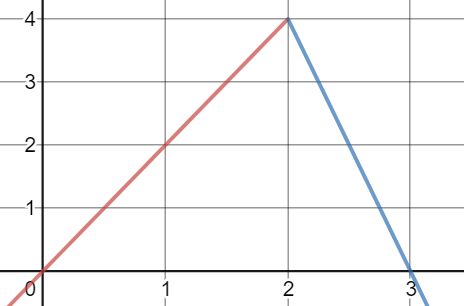
\includegraphics[width=1.5in]{10-19P_functions.png}
                \end{center}
        \end{minipage}
        \begin{enumerate}[(a)]
        \item Let $h(x) = g(f(x))$. Find $h'(3)$.\\
                \textcolor{blue}{
                  \begin{proof}[Computation]
                          The Chain Rule says that $h'(x) = g'(f(x)) \cdot f'(x)$, so
                          \[
                                  h'(3) = g'(f(3)) \cdot f'(3) = g'(1)\cdot 6 = 2 \cdot 6 = 12.
                          \]
                  \end{proof}
                }
        \item Let $k(x) = f(g(x))$. Find $k'(1)$.
                \vfill
        \end{enumerate}
\end{exercise}

\begin{exercise}
        If $F(x) = \sqrt{x^4+3}$, use the Chain Rule to find and simplify $F'(x)$.
        \vfill
\end{exercise}

\newpage

\begin{exercise}
        \begin{enumerate}[(a)]
        \item If $y = e^{x^2}$, compute $\dfrac{dy}{dx}$.
                \vfill
        \item If $z = e^{\tan t}$, compute $\dfrac{dz}{dt}$.
                \vfill
        \end{enumerate}
\end{exercise}

You may need to use the Chain Rule multiple times:
\begin{exercise}
        Find and simplify $G'(x)$ if $G(x) = \sin\left( \sqrt{x^2+2} \right) + e^{\cos(4x)}$.
        \vfill
\end{exercise}

        
\end{document}
